\documentclass{beamer}

\mode<presentation> {
\usetheme{Madrid}
\usecolortheme{whale}
}
\usepackage{lmodern}
\usepackage{graphicx} 
\usepackage{booktabs} 
\usepackage[spanish,es-noquoting,es-lcroman]{babel}
\usepackage[utf8]{inputenc}
\usepackage[T1]{fontenc}
\selectlanguage{spanish}

\title[Título]{Presentacion Moogle!}

\author{Mauricio Sunde Jimenez C111}
\institute[UGR]{
Universidad de La Habana
}
\date{Julio 2023}


\begin{document}

%% Diapositiva de título.
\begin{frame}
\titlepage
\begin{figure}[h]
	\center
    
\includegraphics[width=3cm]{Pictures For Moogle!/matcom.jpg}
    \label{fig:logo}
\end{figure}
\end{frame}

\begin{abstract}
	Moogle! es una aplicacion cuyo proposito es buscar inteligentemente un texto en un conjunto de documentos. Es una aplicacion web, desarrollada con tecnologia .NET Core 6.0, especificamente usando Blazor como *framework* web para la interfaz grafica, y en el lenguaje CSharp.

\begin{figure}[h]
	\center
    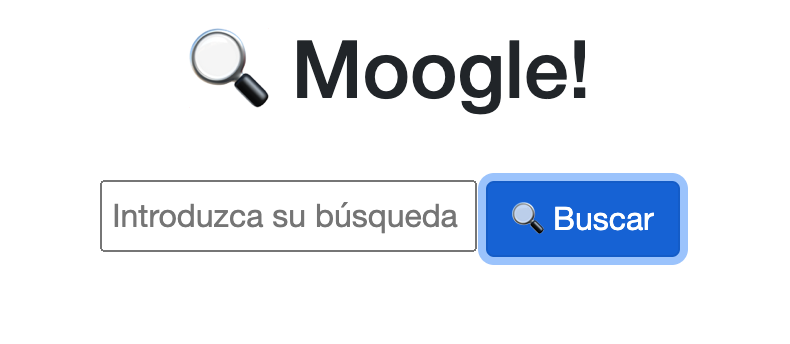
\includegraphics[width=8cm]{Pictures For Moogle!/Picture1.png}
    \label{fig:logo}
\end{figure}

\end{abstract}


%% Diapositiva de contenidos.
% Throughout your presentation, if you choose to use \section{} and \subsection{} commands, 
% these will automatically be printed on this slide as an overview of your presentation
\begin{frame}
\frametitle{Indice} 
\tableofcontents
\end{frame}

\section{Introduccion}

\begin{frame}{Introduccion}
	Moogle! es una aplicación cuyo propósito es buscar inteligentemente un texto en un conjunto de documentos. Esta aplicación dada una query (texto a buscar) del usuario muestra en pantalla los documentos más importantes donde esa query aparece. La idea está en que la búsqueda sea lo más inteligente posible por eso no nos limitamos a solo mostrar exactamente el documento donde aparece exactamente esa query. Moogle implementa un algoritmo de búsqueda, muestra además sugerencias en caso de que la palabra introducida lo necesite, etc. Todo esto será explicado a detalle más adelante.
\end{frame}

\begin{frame}{Explicacion General}
	Para poder obtener la relevancia de cada documento respecto a la búsqueda se ha utilizado la medida de recuperación de información de modelo vectorial y el valor TFIDF. Con este modelo vectorial vemos a los documentos y la Query como vectores que almacenaran sus valores TF-IDF respectivos. El TF-IDF no es más que la frecuencia de ocurrencia del término en la colección de documentos, la cual es una medida numérica que expresa cuán relevante es una palabra para un documento en una colección. Este valor aumenta proporcionalmente al número de veces que una palabra aparece en el documento, pero es compensada por la frecuencia de la palabra en la colección de documentos, lo que permite manejar el hecho de que algunas palabras son generalmente más comunes que otras. Con estos valores podemos verificar que tan parecidos son estos dos vectores mediante la Similitud del coseno. Esta es una medida de la similitud existente entre dos vectores en un espacio que posee un producto interior con el que se evalúa el valor del coseno del ángulo comprendido entre ellos. De esta manera mientras más cercano a 1 son los valores más cercanos a 0 es el ángulo existente entre los dos vectores y más parecidos son estos.
\end{frame}

\begin{frame}
\frametitle{Como usar Moogle!}
\begin{block}{1}
	Ingrese la palabra deseada a buscar en el campo de busqueda que dice Introduzca su busqueda, autoseguido haga click en Buscar.
\end{block}

\begin{block}{2}
	Su busqueda aparecera en el lado izquerdo en orden descendente de relevancia por lo tanto el primer resultado es donde mas relevancia tiene la palabra buscada ademas de un fragmento de texto donde aparece dicha palabra
\end{block}

\begin{block}{3}
	Si la palabra buscada no se encuentra entonces aparecera una sugerencia en base a lo mas proximo que usted desea buscar si se hace click en dicha sugerencia se iniciara otra busqueda con esa nueva palabra
\end{block}
\end{frame}

\section{Explicacion General}
\section{Como usar Moogle!}
\section{Imagenes sobre el Moogle!}

\begin{frame}{Imagenes sobre el Moogle!}
	\begin{figure} [h]
		\center
		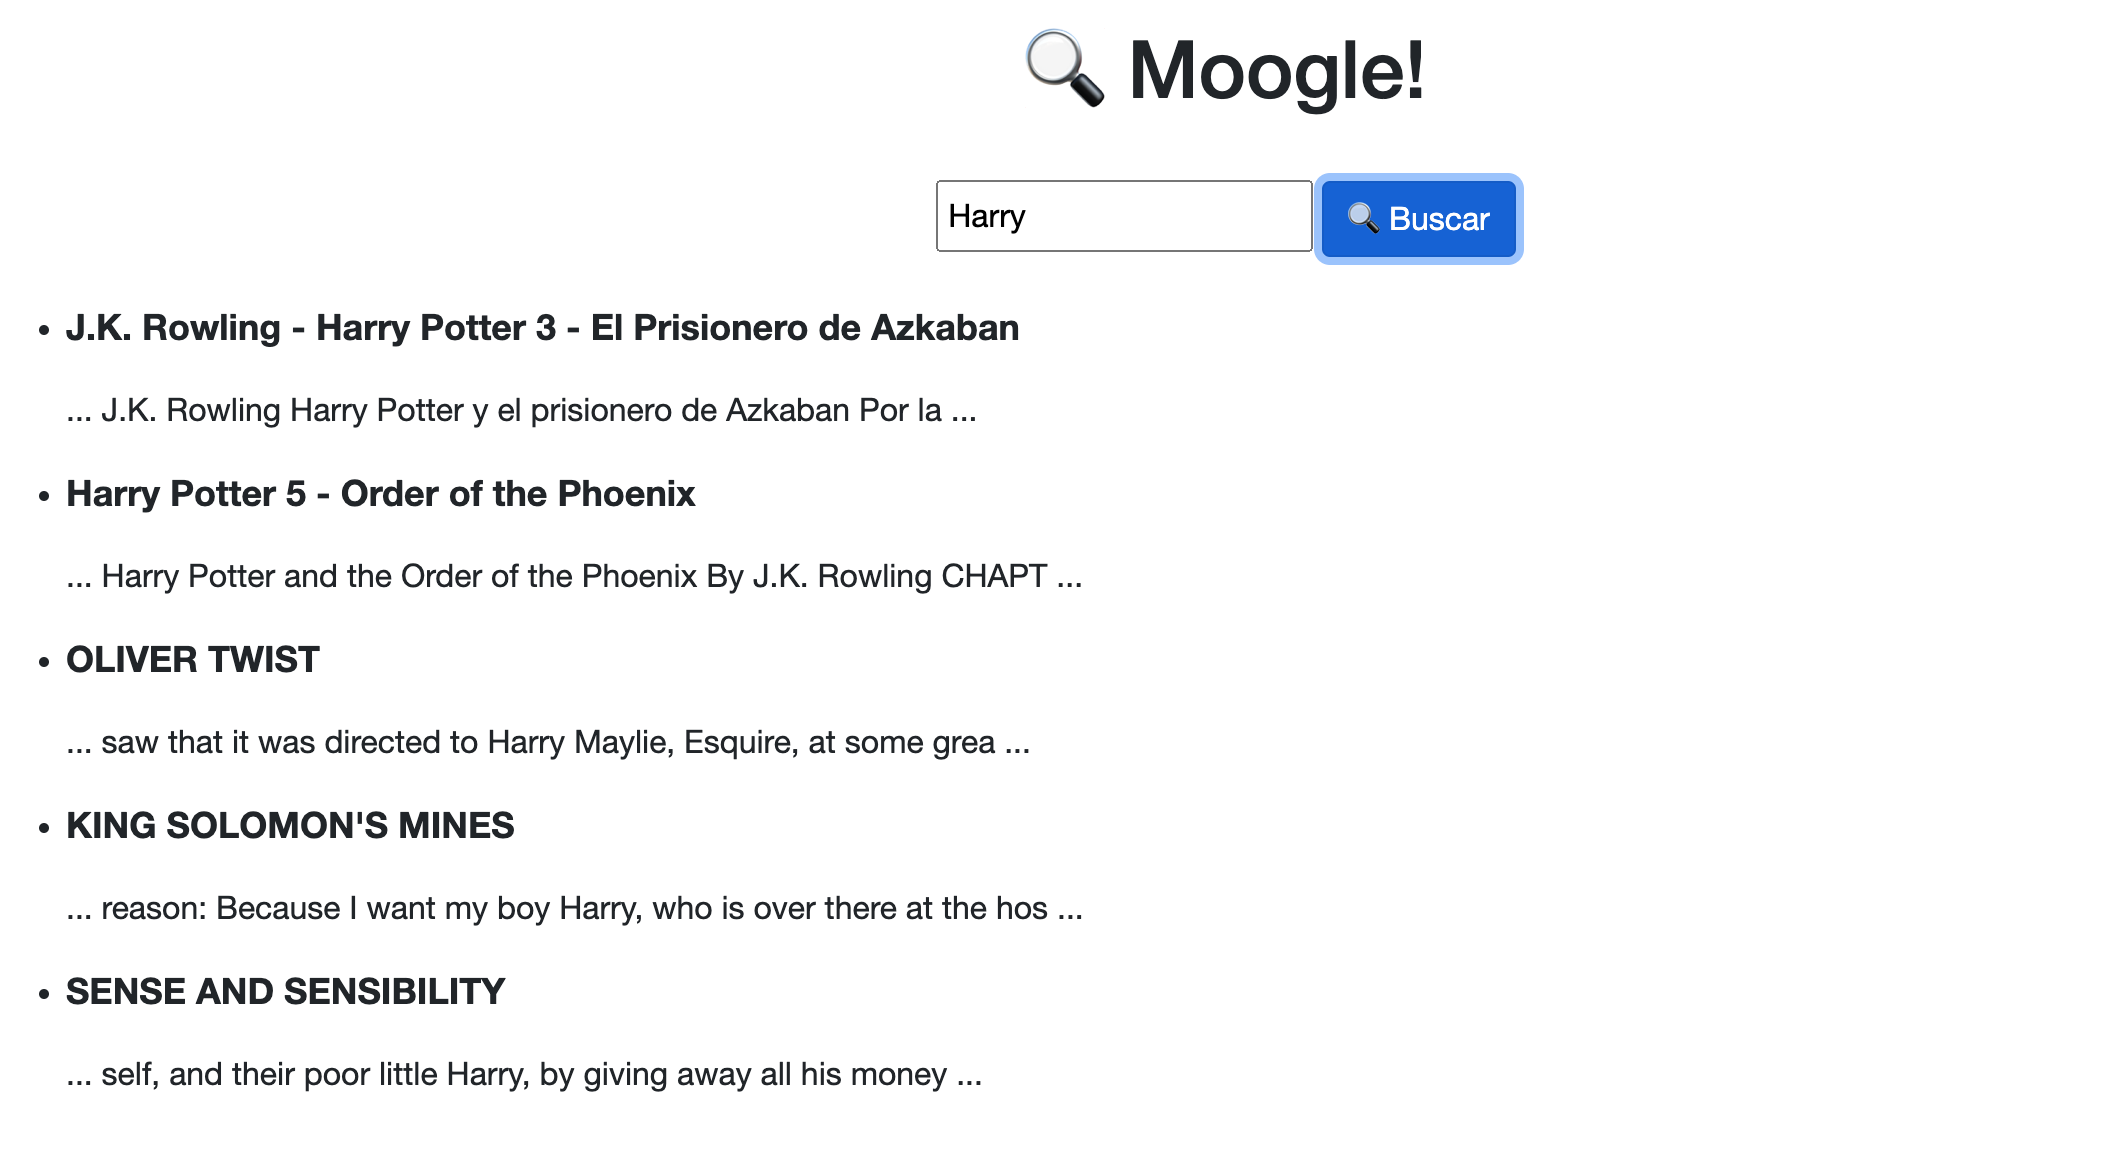
\includegraphics[width=10cm]{Pictures For Moogle!/Picture2.png}
		\caption{Busqueda realizada con exito y con un fragmento del texto donde la palabra buscada aparece}
		\label{fig:logo}
	\end{figure}
\end{frame}

\begin{frame}{Imagenes sobre el Moogle!}
	\begin{figure} [h]
		\center
		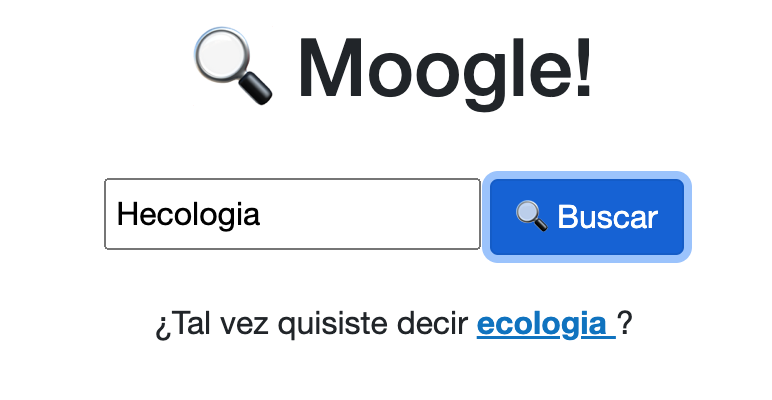
\includegraphics[width=10cm]{Pictures For Moogle!/Picture3.png}
		\caption{Ejemplo que muestra la sugerencia}
		\label{fig:logo}
	\end{figure}
\end{frame}

\begin{frame}{Imagenes sobre el Moogle!}
	\begin{figure} [h]
		\center
		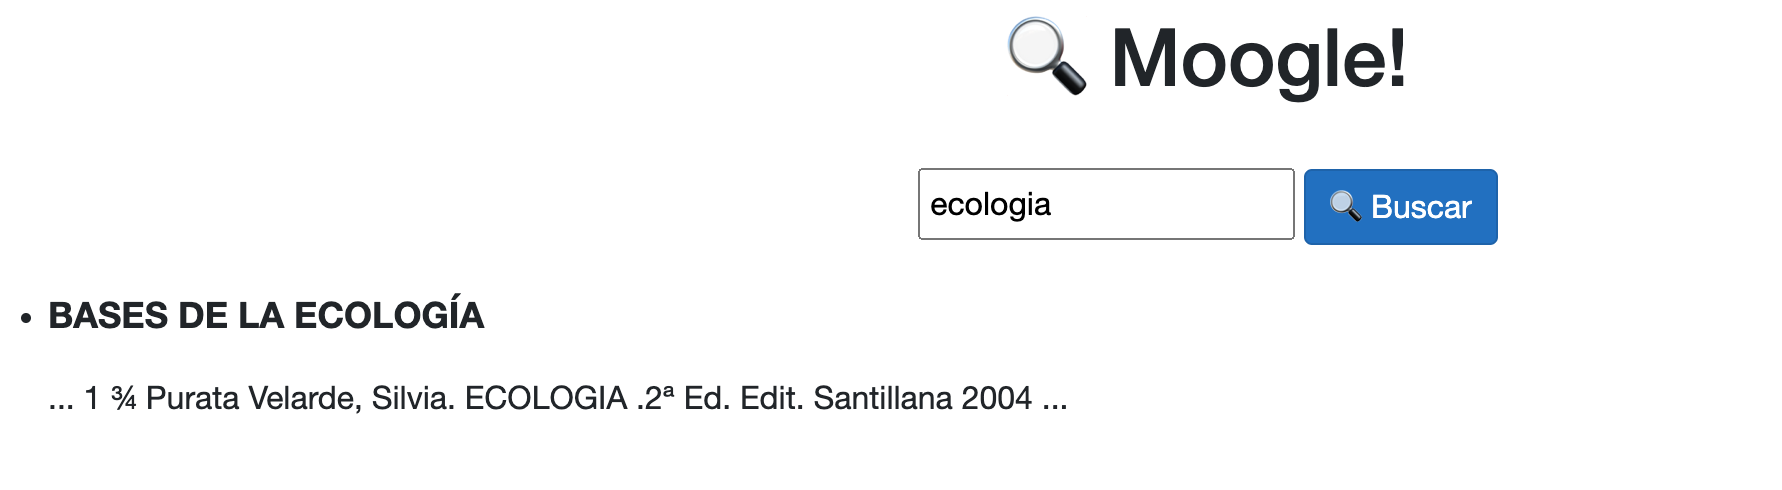
\includegraphics[width=10cm]{Pictures For Moogle!/Picture4.png}
		\caption{Nueva Busqueda}
		\label{fig:logo}
	\end{figure}
\end{frame}

\begin{frame}
\Huge{\centerline{Fin.}}
\end{frame}

\end{document} 